\section{Referencia de la Clase Clients\-List}
\label{classClientsList}\index{ClientsList@{ClientsList}}
Administra la lista de clientes.  


{\tt \#include $<$clientslist.h$>$}

Diagrama de colaboraci\'{o}n para Clients\-List:\begin{figure}[H]
\begin{center}
\leavevmode
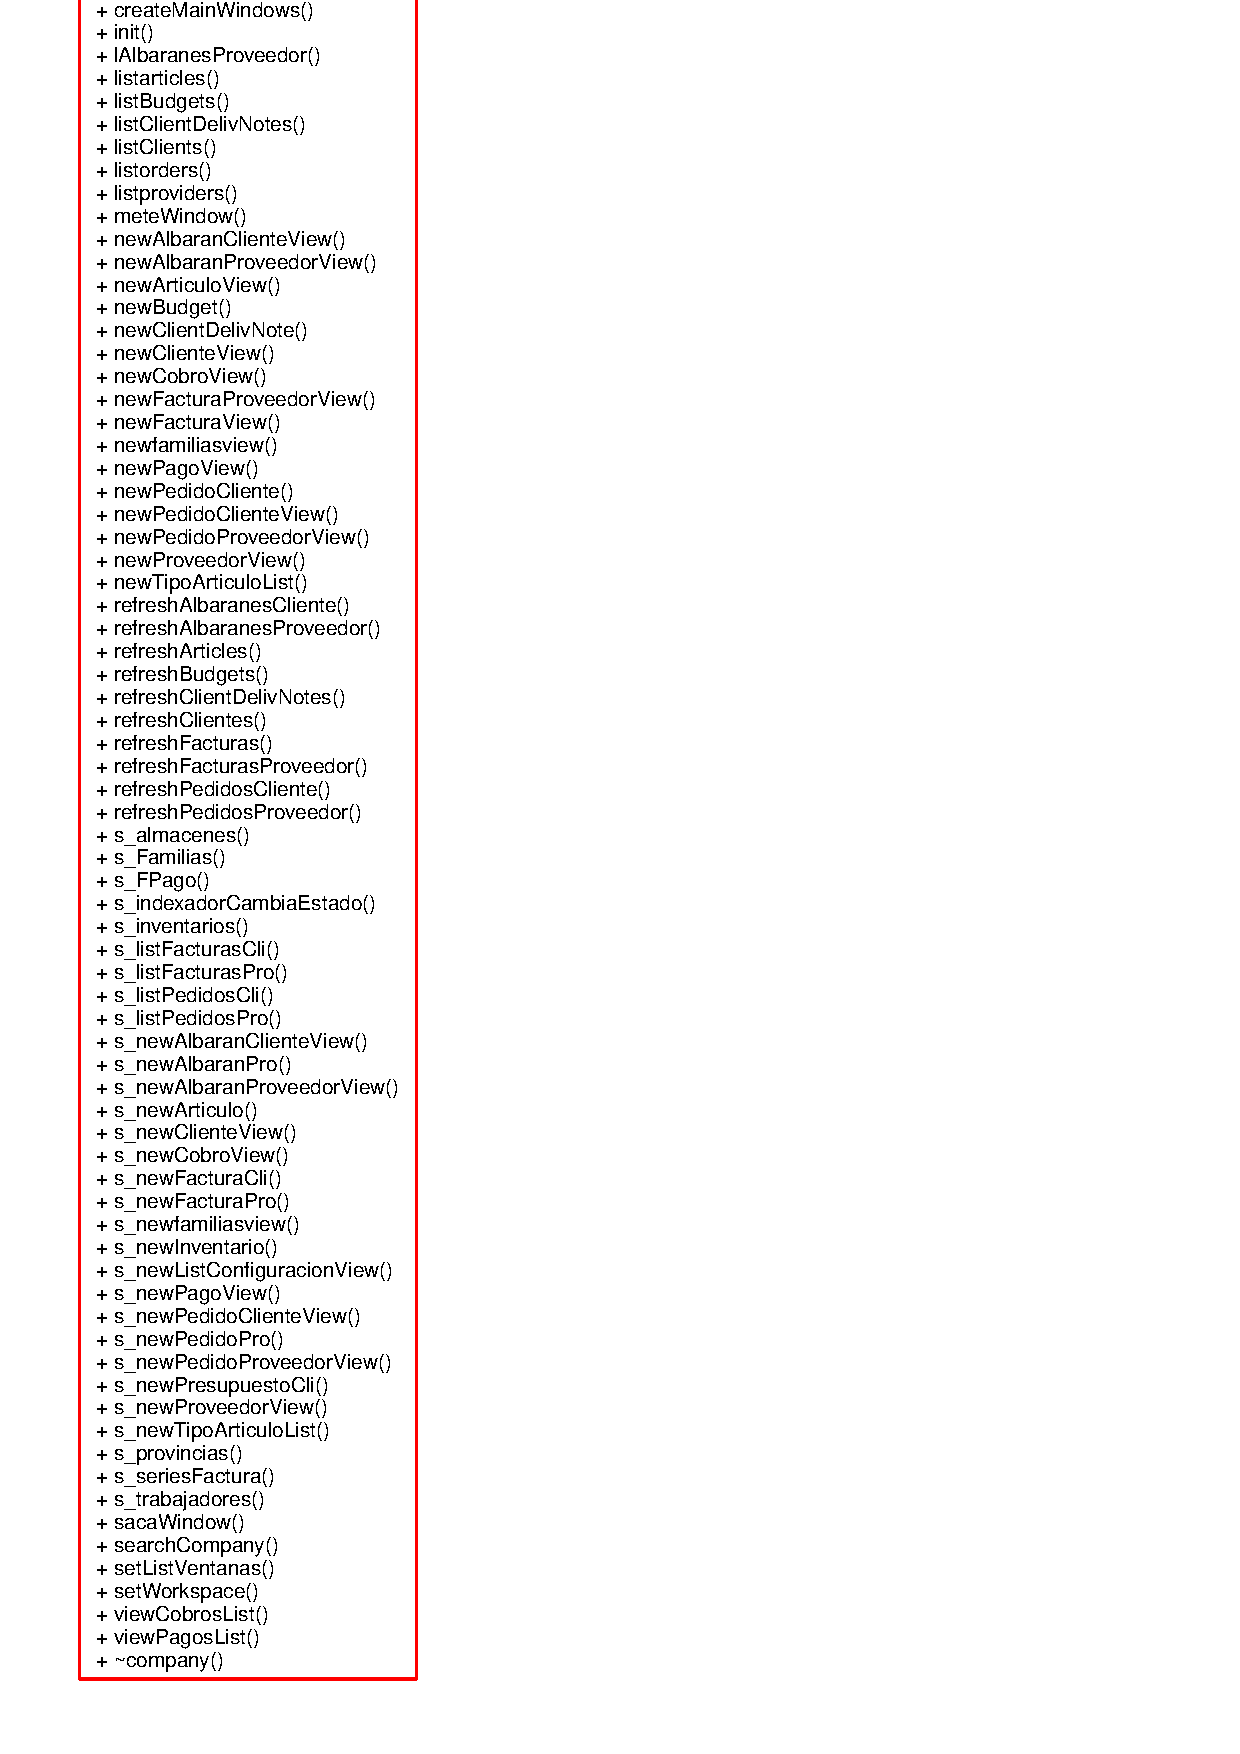
\includegraphics[width=117pt]{classClientsList__coll__graph}
\end{center}
\end{figure}
\subsection*{Tipos p\'{u}blicos}
\begin{CompactItemize}
\item 
enum {\bf edmode} \{ {\bf Edit\-Mode} =  0, 
{\bf Select\-Mode} =  1
 \}
\end{CompactItemize}
\subsection*{Slots p\'{u}blicos}
\begin{CompactItemize}
\item 
virtual void {\bf on\_\-m\_\-filtro\_\-text\-Changed} (const QString \&text)\label{classClientsList_i0}

\item 
virtual void {\bf on\_\-mui\_\-actualizar\_\-clicked} ()\label{classClientsList_i1}

\item 
virtual void {\bf on\_\-mui\_\-borrar\_\-clicked} ()\label{classClientsList_i2}

\item 
virtual void {\bf on\_\-mui\_\-configurar\_\-toggled} (bool checked)\label{classClientsList_i3}

\item 
virtual void {\bf on\_\-mui\_\-crear\_\-clicked} ()\label{classClientsList_i4}

\item 
virtual void {\bf on\_\-mui\_\-editar\_\-clicked} ()\label{classClientsList_i5}

\item 
virtual void {\bf on\_\-mui\_\-exportar\_\-clicked} ()\label{classClientsList_i6}

\item 
virtual void {\bf on\_\-mui\_\-importar\_\-clicked} ()\label{classClientsList_i7}

\item 
virtual void {\bf on\_\-mui\_\-imprimir\_\-clicked} ()\label{classClientsList_i8}

\item 
virtual void {\bf on\_\-mui\_\-informeclientes\_\-clicked} ()\label{classClientsList_i9}

\item 
void {\bf on\_\-mui\_\-list\_\-item\-Double\-Clicked} (QTable\-Widget\-Item $\ast$)\label{classClientsList_i10}

\end{CompactItemize}
\subsection*{Se\~{n}ales}
\begin{CompactItemize}
\item 
void {\bf selected} (QString)\label{classClientsList_l0}

\end{CompactItemize}
\subsection*{M\'{e}todos p\'{u}blicos}
\begin{CompactItemize}
\item 
QString {\bf cifclient} ()\label{classClientsList_a0}

\item 
{\bf Clients\-List} ({\bf company} $\ast$, QWidget $\ast$parent=0, Qt::WFlags flag=0, edmode editmode=Edit\-Mode)
\item 
void {\bf editar} (int)\label{classClientsList_a2}

\item 
void {\bf edit\-Mode} ()\label{classClientsList_a3}

\item 
void {\bf hide\-Botonera} ()\label{classClientsList_a4}

\item 
void {\bf hide\-Busqueda} ()\label{classClientsList_a5}

\item 
QString {\bf idclient} ()\label{classClientsList_a6}

\item 
QString {\bf nomclient} ()\label{classClientsList_a7}

\item 
void {\bf presenta} ()
\item 
void {\bf select\-Mode} ()\label{classClientsList_a9}

\item 
void {\bf show\-Botonera} ()\label{classClientsList_a10}

\item 
void {\bf show\-Busqueda} ()\label{classClientsList_a11}

\end{CompactItemize}
\subsection*{Atributos p\'{u}blicos}
\begin{CompactItemize}
\item 
{\bf company} $\ast$ {\bf m\_\-companyact}\label{classClientsList_o0}

\end{CompactItemize}


\subsection{Descripci\'{o}n detallada}
Administra la lista de clientes. 



\subsection{Documentaci\'{o}n del constructor y destructor}
\index{ClientsList@{Clients\-List}!ClientsList@{ClientsList}}
\index{ClientsList@{ClientsList}!ClientsList@{Clients\-List}}
\subsubsection{\setlength{\rightskip}{0pt plus 5cm}Clients\-List::Clients\-List ({\bf company} $\ast$ {\em comp}, QWidget $\ast$ {\em parent} = {\tt 0}, Qt::WFlags {\em flag} = {\tt 0}, edmode {\em editmode} = {\tt EditMode})}\label{classClientsList_a1}


Si estamos en el modo edicion metemos la ventana en el lugar apropiado. 

\subsection{Documentaci\'{o}n de las funciones miembro}
\index{ClientsList@{Clients\-List}!presenta@{presenta}}
\index{presenta@{presenta}!ClientsList@{Clients\-List}}
\subsubsection{\setlength{\rightskip}{0pt plus 5cm}void Clients\-List::presenta ()}\label{classClientsList_a8}


Iniciamos los clientes. Hacemos la consulta a la base de datos y presentamos el listado. 

La documentaci\'{o}n para esta clase fu\'{e} generada a partir de los siguientes archivos:\begin{CompactItemize}
\item 
clientslist.h\item 
clientslist.cpp\end{CompactItemize}
